\DiaryEntry{Exponential Distribution, 1}{2019-08-30}{Stochastic}

The exponential distribution is given by

\bee
f(x) = \lambda e^{- \lambda x}, \quad x \geq 0
\eee

with corresponding CDF

\bee
F(x) = P(X < x) = \int_{t=0}^x \lambda e^{- \lambda t} dt = \left. -e^{-\lambda t} \right|_{t=0}^x = 1 - e^{-\lambda x}
\eee

and complementary cdf

\bee
\bar F(x) = P(X > x) = e^{-\lambda x} 
\eee


For completeness, we note that the mean $E(X)$ is given by

\begin{align*}
E(X) &= \int_{t=0}^\infty x \lambda e^{- \lambda x} dx = \lambda \int_{t=0}^\infty x e^{- \lambda x} dx = \lambda \left( -\frac{1}{\lambda} x e^{-\lambda x} \left. \right|_{x=0}^\infty + \int_{t=0}^\infty \frac{1}{\lambda} e^{- \lambda x} dx \right) \\
&= \lambda \left( 0 + \frac{1}{\lambda}  \int_{t=0}^\infty e^{- \lambda x} dx \right) = \cdots = \frac{1}{\lambda}
\end{align*}

where we used partial integration with $u' = e^{-\lambda x}$ and $v = x$. Then $u = -\frac{1}{\lambda}e^{-\lambda x}$, and $v' = 1$.

The variance calculation seems to be even more messier ($\int x^2 \lambda e^{-\lambda x}dx$), let us go via the moment generating function (MGF) instead. The MGF $M_X(t)$ is defined according to

\bee
M_X(t) = E(e^{t X}) = \int_{x=0}^\infty e^{tx} \lambda e^{-\lambda x} dx = \lambda \int_{x=0}^\infty e^{(t - \lambda) x} dx = \frac{1}{t - \lambda} e^{x(t-\lambda)}\left. \right|_{x=0}^\infty = \frac{\lambda}{\lambda-t} \qed
\eee

We can use the MGF to calculate moments as follows,

\bee
E{X^n} = \frac{d^n M_X(t)}{dt^n}\left. \right|_{t=0}
\eee

and for the exponential distribution we have (using Maxima)

\bee
E(X^2) = \frac{d^2 M_X(t)}{dt^2}\left. \right|_{t=0} = \frac{2 \lambda}{(\lambda-t)^3}\left. \right|_{t=0} = \frac{2}{\lambda^2}
\eee

The variance is then

\bee
E(X^2) - E^2(X) = \frac{2}{\lambda^2} - \frac{1}{\lambda^2} = \frac{1}{\lambda^2} \qed
\eee

The exponential distribution has the memoryless property (it is the only continuous distribution with this property),

\bee
P(X > s+t | X > s) = \frac{P(X > s+t)}{P(X>s)} = \frac{e^{-\lambda (s+t)}}{e^{-\lambda s}} = e^{-\lambda t} = P(X > t)
\eee

We can understand this by interpreting $X$ as a the lifetime of a device. Modeling $X$ as memoryless means that the probability for the device surving another $t$ seconds after it has already survived $s$ seconds of operation is the same as the probability that the device has survived $t$ seconds (independent of $s$).

We can extend this by introducing the \emph{failure rate function} $r(t)$ as follows,

\bee
r(t) = \frac{f(t)}{\bar F(t)}
\eee

We can interpret this expression by considering the probability that a $t$-year old item will fail during the next $dt$ seconds

\bee
P(X \in (t + dt) | X > t) = \frac{P(X \in (t + dt))}{P(X>t)} \approx \frac{f(t) dt}{\bar F(t)} = r(t) dt
\eee

and therefore $r(t)$ is the instantenuous failure rate of a $t$-year old item. When $r(t)$ is increasing with $t$, we talk of an increasing failure rate. The longer the device has survived, the more likely a failure becomes. This is the case with an old car where we expect (more) issues after a certain lifespan.

When $r(t)$ is decreasing with $t$, we talk of a decreasing failure rate. The longer the device has survived, the less likely it is to break. This is the case in chip fabrication where chips tend to fail early on and when they have survided this phase, are less likely to fail.

The middle case of a constant failure rate function yields an exponential distribution.


\subsection{Interesting Properties}

The exponential distribution has a number of nice properties which we discuss in the following.

\paragraph{Probability of $X_1 < X_2$.}. We consider two RVs with an exponential distribution and parameter $\lambda_1, \lambda_2$, respectively. We calculate the probability $P(X_1 < X_2)$ as follows,

\bee
P(X_1 < X_2) = \int_{a=0}^\infty P(X_1 < X_2 | X_2 = a) f_2(a) da = \int_{a=0}^\infty (1 - e^{-\lambda_1 a}) \lambda_2 e^{-\lambda_2 a} da = \cdots = \frac{\lambda_1}{\lambda_1 + \lambda_2}
\eee

\paragraph{Probability of $X_1 > X_2$.} Same setup, different probability,

\bee
P(X_1 > X_2) = \int_{a=0}^\infty P(X_1 > X_2 | X_2 = a) f_2(a) da = \int_{a=0}^\infty e^{-\lambda_1 a} \lambda_2 e^{-\lambda_2 a} da = \cdots = \frac{\lambda_2}{\lambda_1 + \lambda_2}
\eee

\paragraph{Distribution of Minimum.} Now we define a new RV $X$ as

\bee
X = \min (X_1, X_2)
\eee 

We calculate the CCDF $P(X > t)$ as

\begin{align*}
P(X > t) &= P( \min(X_1, X_2) > t) = P( X_1 > t \, \text{and} \, X_2 > t) = P(X_1 > t) P(X_2 > t) \\ &= e^{-\lambda_1 t} e^{-\lambda_2 t} = e^{- (\lambda_1 + \lambda_2)t}
\end{align*}

where we have used the fact for being $X_1$ and $X_2$ independent. The CCDF is the CCDF of an exponential distribution with parameter $\lambda_1 + \lambda_2$. So

\bee
X = \min (X_1, X_2) \sim \text{Exponential}(\lambda_1 + \lambda_2)
\eee

This can be generalized to the case of $n$ exponential RVs,

\bee
X = \min (X_1, X_2, \ldots, X_n)
\eee

which has CCDF

\bee
P(X > t) = P(X_1 > t) \cdots P(X_n > t) = e^{-\lambda_1 t} \cdots e^{-\lambda_n t} = e^{-(\lambda_1 + \cdots \lambda_n) t}
\eee

which is an exponential RV with parameter $\lambda_1 + \cdots \lambda_n$.

\paragraph{Distribution of Maximum.} Now we define a new RV $X$ as

\bee
X = \max (X_1, X_2)
\eee 

In this case the CDF can be expressed simply; we have

\begin{align*}
P(X < t) &= P( X_1 < t \, \text{and} \, X_2 < t) = P(X_1 < t) P(X_2 < t) \\
&= (1-e^{-\lambda_1 t})(1-e^{-\lambda_2 t}) = 1 - e^{-\lambda_1 t} - e^{-\lambda_2 t} + e^{-(\lambda_1 + \lambda_2)t}
\end{align*}

This looks nice for sure, but is not an exponential distribution. We can calculate the pdf according to

\bee
f_X(t) = \lambda_1 e^{-\lambda_1 t} + \lambda_2 e^{-\lambda_2 t} + (\lambda_1 + \lambda_2) e^{-(\lambda_1 + \lambda_2)t}
\eee

which (also) shows that this is not an exponential distribution. The mean is

\bee
E(X) = \frac{1}{\lambda_1} + \frac{1}{\lambda_2} - \frac{1}{\lambda_1 + \lambda_2}
\eee

When the $\lambda$s differ much in size, say $\lambda_2 \gg \lambda_1$, the distribution for $X_2$ falls off much steeper and the maximum $X$ is dominated by $X_1$. In this case we can approximate $X$ for large values with an exponential distribution

\bee
f_X(t) \approx \lambda_1 e^{- \lambda_1 t}
\eee

This is shown in the following Figure for $\lambda_1=0.5, \lambda_2=5$.

The notable difference however, is that $f_X(0) = 0$ which does not hold true for the exponential distribution. In scenarios where this is important, the approximation will fail. 


\begin{figure}[hbt!]
\centering
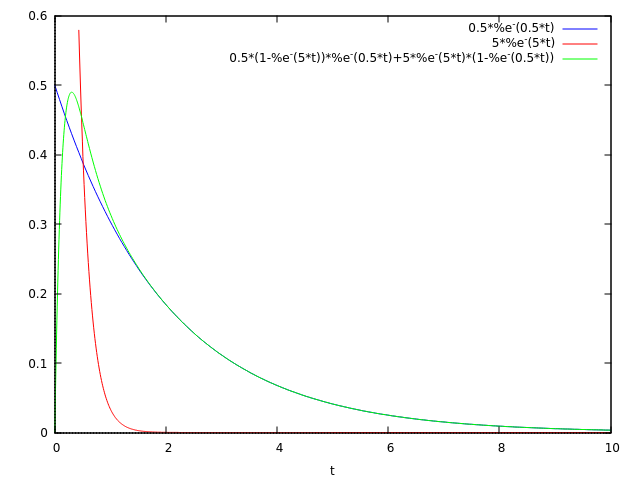
\includegraphics[scale=0.5]{images/exp_pdf_1_1.png}
\end{figure}



\paragraph{Sum of two exponential RVs.} Now consider

\bee
Z = X_1 + X_2
\eee

and obtain the pdf by convolving the two pdfs,

\begin{align*}
f_Z(z) &= \int_{x=0}^z f_{X_1}(x) f_{X_2}(z - x) dx = \int_{x=0}^z \lambda_1 e^{-\lambda_1 x} \lambda_2 e^{-\lambda_2(z-x)} dx \\ &= \lambda_1 \lambda_2 e^{-\lambda_2 z} \int_{x=0}^z e^{-\lambda_1 x + \lambda_2 x} dx = \cdots \frac{\lambda_1 \lambda_2}{\lambda_2 - \lambda_1} \left( e^{-\lambda_1 z} - e^{-\lambda_2 z} \right)
\end{align*}

Slightly different is the case when $\lambda_1 = \lambda_2 = \lambda$. We have

\bee
f_Z(z) = \lambda^2 e^{-\lambda z} \int_{x=0}^z e^{-\lambda x} e^{\lambda x} dx = \lambda^2 z e^{-\lambda z}
\eee

%%% Local Variables:
%%% mode: latex
%%% TeX-master: "journal"
%%% End:
